\subsubsection{Heldout}
\label{subsubsec:heldout-res}

In Table~\ref{tab:heldout-map-ndcg-table} are reported the \ac{nDCG} and \ac{MAP} values obtained from the submitted runs on the heldout collection, while in Figure~\ref{fig:precision-recall-curve-heldout} is reported the interpolated Precision-Recall curve. Comparing these results with the ones obtained on training, shown in Table~\ref{tab:map-ndcg-table} and Figure~\ref{fig:precision-recall-curve} respectively, we can see that every run suffered a \emph{performance drop} over all the measures. This worsening was \emph{expected} and it can be due to the fact that the system has been tuned over a different set of queries. It should also be noticed that this set of queries is more than 6 times smaller compared to the training one, therefore the presence of some \emph{outliers} could have caused the mean performances to drop and to not be a good descriptor of the system.

Observing the \ac{nDCG} and \ac{AP} boxplots, shown in Figure~\ref{fig:heldout-boxplot}, we can notice that the runs performed on the French collection have a similar structure in terms of median values and interquartile ranges. We can also notice that, in the \ac{AP} boxplot, the reranked runs fr\_1, fr\_2 have longer whiskers, while the others show the presence of outliers.

From the ANOVA2 analysis, which results are reported in Table~\ref{tab:heldout-anova2}, we can see that $p\textrm{--}value>\alpha$, therefore we \emph{cannot reject} the null hypothesis. Moreover, from Tukey's \ac{HSD} multiple comparison shown in Figure~\ref{fig:heldout-hsd}, we can derive that the French runs can be considered to be similar to each other.

\begin{table}[tbp]
\caption{\ac{nDCG} and \ac{MAP} values on heldout collection}
  \label{tab:heldout-map-ndcg-table}
    \centering
    \begin{tabular}{|p{0.7\linewidth}|p{0.075\linewidth}|p{0.075\linewidth}|}
	\toprule
	\textbf{Run name} & \textbf{nDCG} & \textbf{MAP} \\
	\midrule
        FADERIC\_French-BM25-Stop50-LightStem-Shingle-Fuzzy-SynCustom-Rerank20W6 & 0.4169 & 0.2474 \\
        FADERIC\_French-BM25-Stop50-LightStem-Shingle-Fuzzy-Rerank30 & 0.4147 & 0.2416 \\
        FADERIC\_French-BM25-Stop50-LightStem-Shingle-Fuzzy-SynCustom & 0.4080 & 0.2376 \\
        FADERIC\_French-BM25Tuned-Stop50-LightStem-Shingle-Fuzzy & 0.4044 & 0.2324 \\
        FADERIC\_English-BM25-Stop50-KStem-Shingle-Fuzzy-SynPOS\\-Rerank30 & 0.3030 & 0.1626 \\
	\bottomrule
    \end{tabular}
\end{table}

\begin{figure}[tbp]
  \centering
  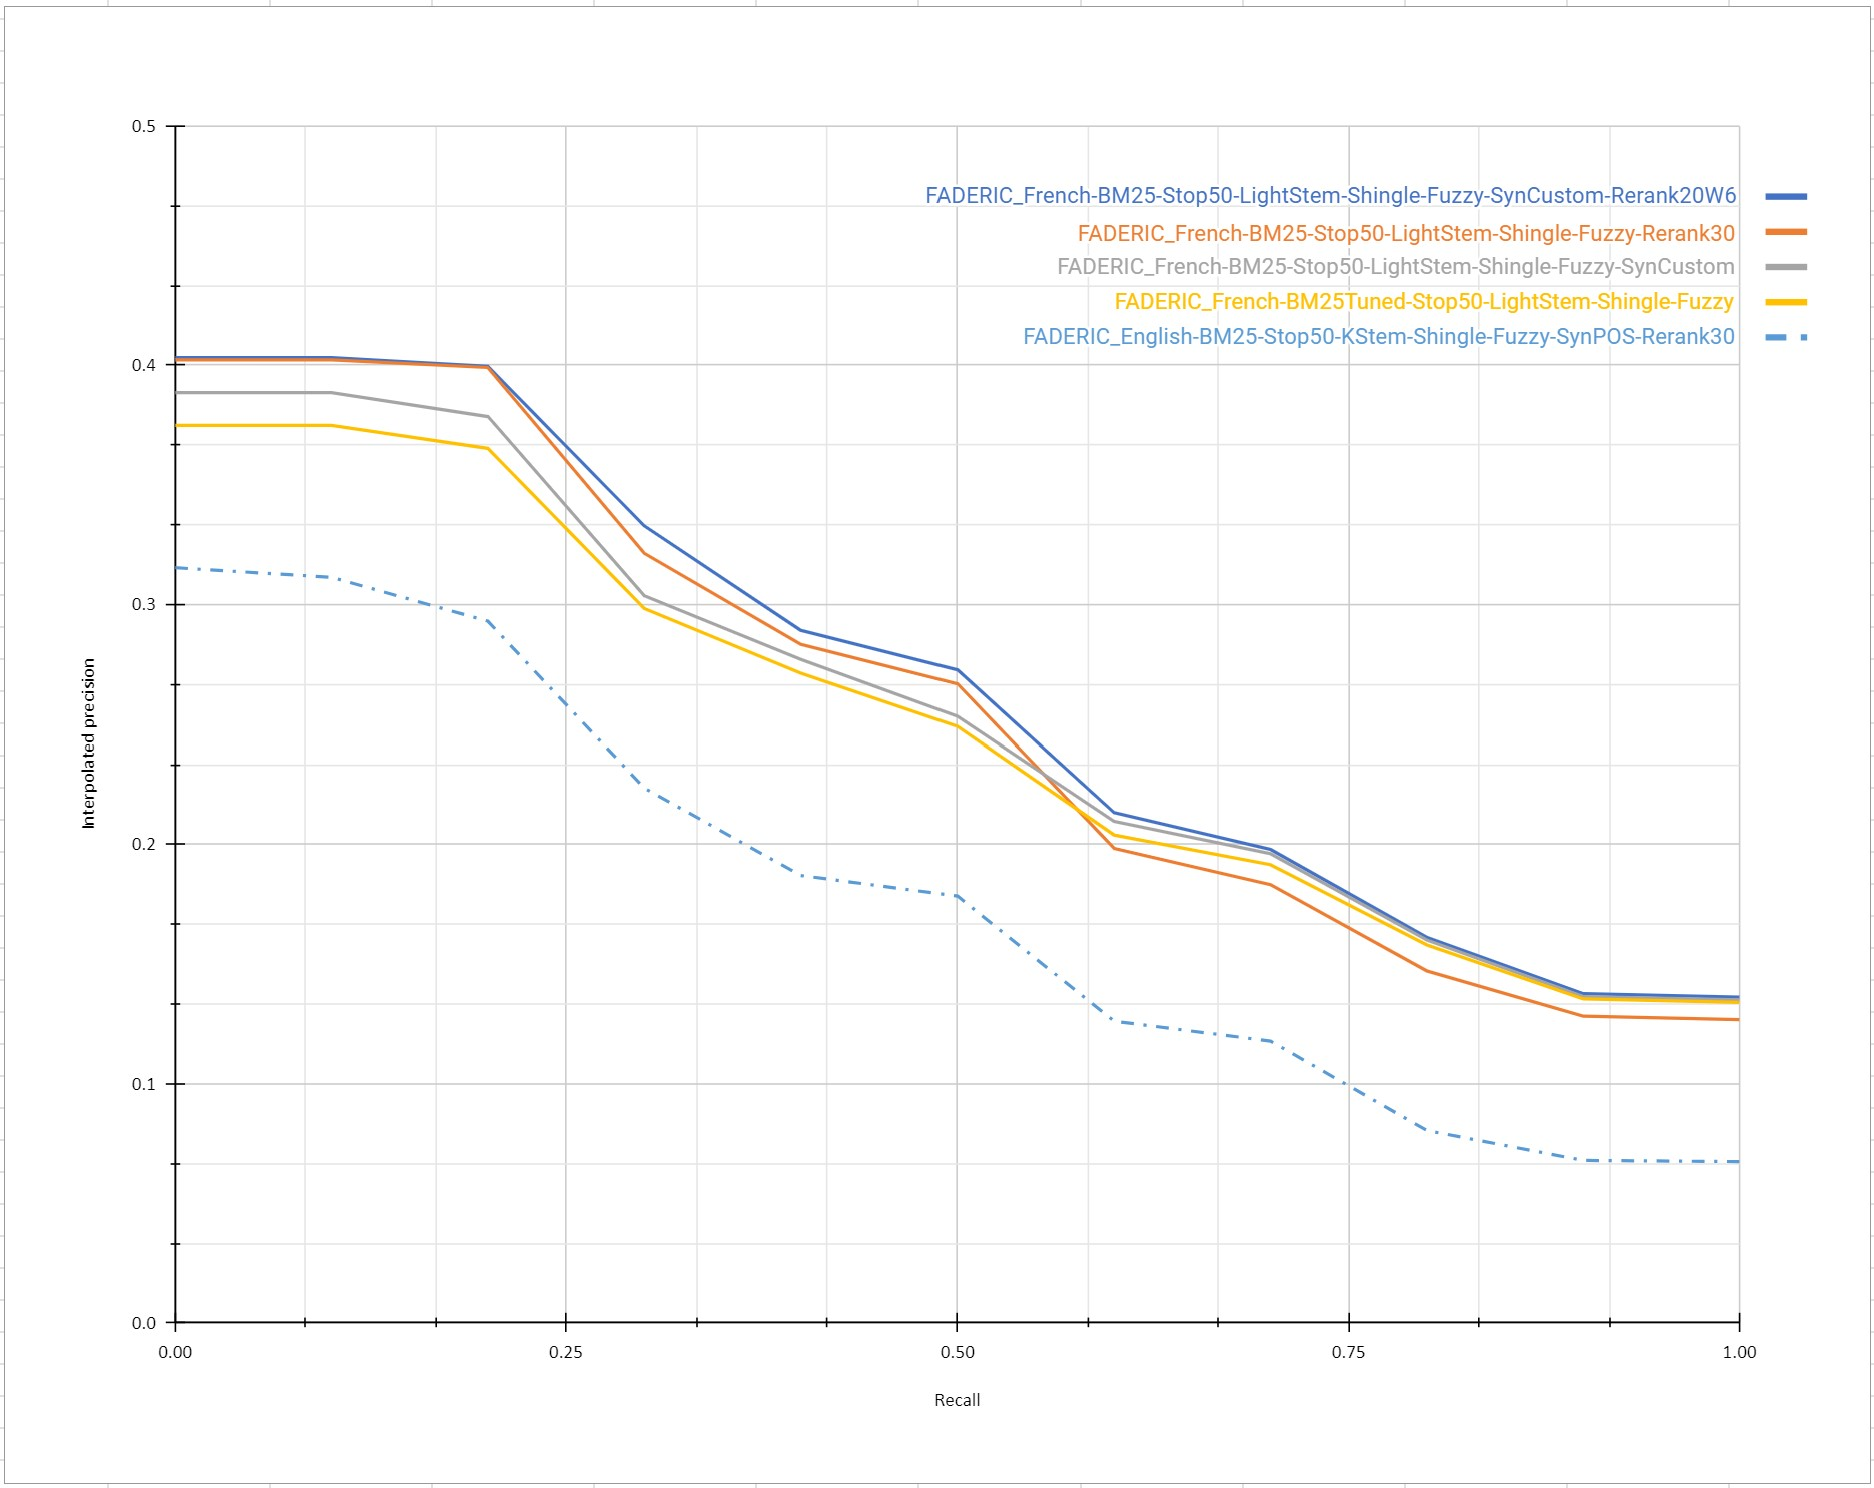
\includegraphics[width=1\linewidth]{figure/iprec-recall-HELDOUT.jpg}
  \caption{Interpolated Precision-Recall curve on heldout collection}
  \label{fig:precision-recall-curve-heldout}
\end{figure}

\begin{figure}[tbp]
     \centering
     \begin{subfigure}[b]{0.45\textwidth}
         \centering
         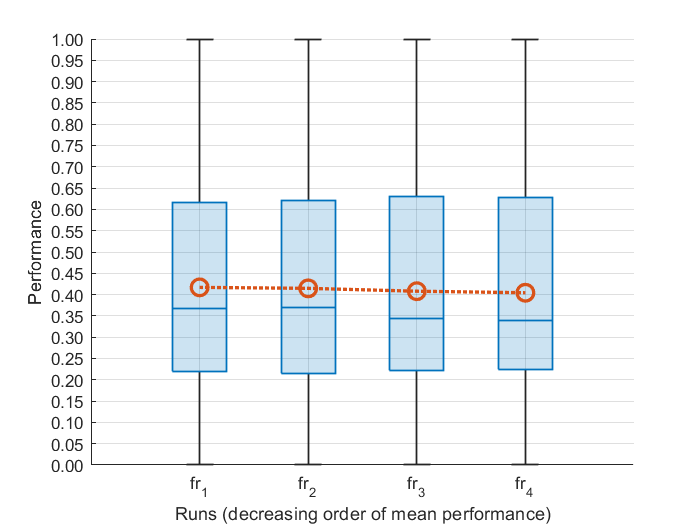
\includegraphics[width=\textwidth]{figure/heldout-ndcg-boxplot.png}
         \caption{\ac{nDCG}}
     \end{subfigure}
     \hfill
     \begin{subfigure}[b]{0.45\textwidth}
         \centering
         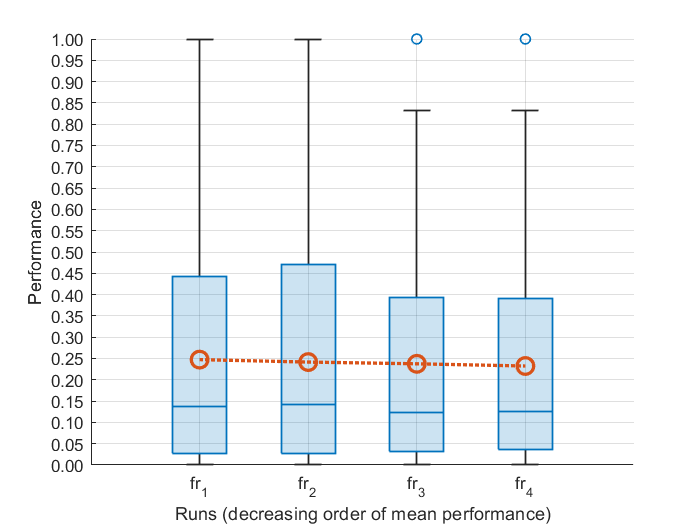
\includegraphics[width=\textwidth]{figure/heldout-map-boxplot.png}
         \caption{\ac{AP}}
     \end{subfigure}
        \caption{Box plot on heldout collection, the mean values are shown in red}
        \label{fig:heldout-boxplot}
\end{figure}

\begin{table}[tbp]
     \caption{ANOVA2 on heldout collection}
    \begin{subtable}[t]{1\textwidth}
        \centering
	\caption{\ac{nDCG}}
	\begin{tabular}{|l|l|l|l|l|l|}
	\toprule
        \textbf{Source} & \textbf{SS} & \textbf{df} & \textbf{MS} & \textbf{F} & \textbf{Prob$>$F} \\
        \midrule
	\textbf{Systems} & 0.01 & 3   & 0.003  & 0.64  & 0.58 \\
	\textbf{Topics}    & 23.54  & 97  & 0.242 & 47.20 & 1.97E-134 \\
	\textbf{Error}   & 1.49  & 291 & 0.005 & - & - \\
	\textbf{Total}   & 25.04  & 391 & - & - & - \\
	\bottomrule
       \end{tabular}
    \end{subtable}
        \begin{subtable}[t]{1\textwidth}
        \centering
	\caption{\ac{AP}}
        \begin{tabular}{|l|l|l|l|l|l|}
	\toprule
        \textbf{Source} & \textbf{SS} & \textbf{df} & \textbf{MS} & \textbf{F} & \textbf{Prob$>$F} \\
        \midrule
	\textbf{Systems} & 0.01 & 3  & 0.003  & 0.68  & 0.55 \\
	\textbf{Topics}    & 23.35  & 97  & 0.240 & 42.10 & 8.26E-128 \\
	\textbf{Error}   & 1.66  & 291 & 0.057 & - & - \\
	\textbf{Total}   & 25.03  & 391 & - & - & - \\
	\bottomrule
       \end{tabular}
    \end{subtable}
     \label{tab:heldout-anova2}
\end{table}

\begin{figure}[tbp]
     \centering
     \begin{subfigure}[b]{0.45\textwidth}
         \centering
         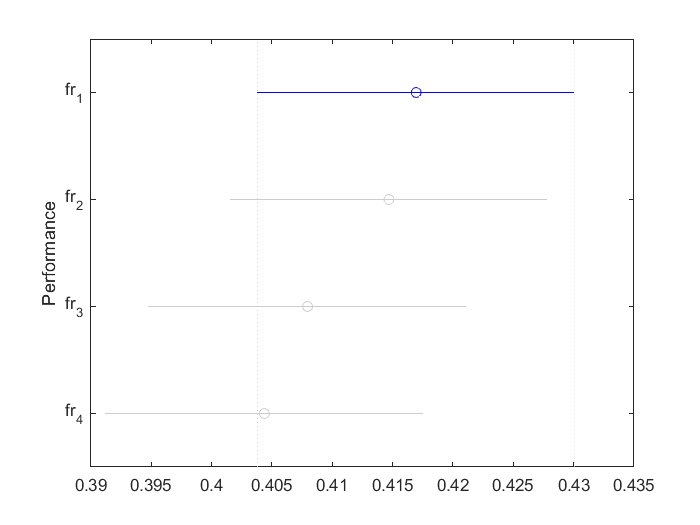
\includegraphics[width=\textwidth]{figure/heldout-ndcg-hsd.png}
	\caption{\ac{nDCG}}
     \end{subfigure}
     \hfill
     \begin{subfigure}[b]{0.45\textwidth}
         \centering
         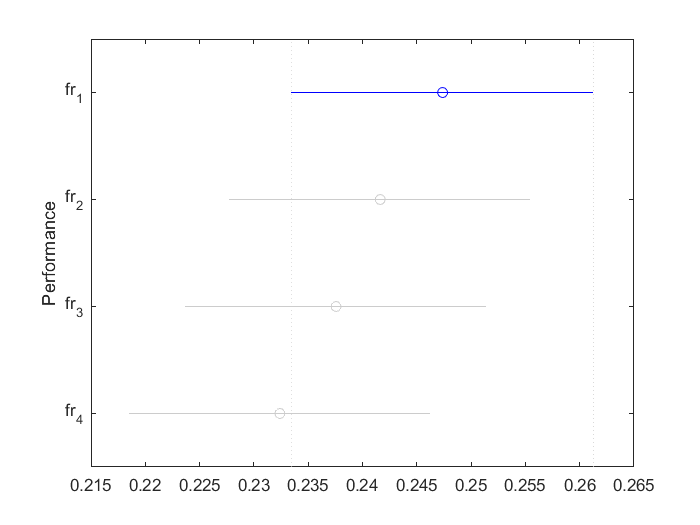
\includegraphics[width=\textwidth]{figure/heldout-map-hsd.png}
	\caption{\ac{AP}}
     \end{subfigure}
        \caption{Tukey's \ac{HSD} on heldout collection}
        \label{fig:heldout-hsd}
\end{figure}